%%%%%%%%%%%%%%%%%%%%%%%%%%%%%%%%%%%%%%%%%%%%%%%%%%%%%%%%%%%%%%%%%%%%%%
% How to use writeLaTeX: 
%
% You edit the source code here on the left, and the preview on the
% right shows you the result within a few seconds.
%
% Bookmark this page and share the URL with your co-authors. They can
% edit at the same time!
%
% You can upload figures, bibliographies, custom classes and
% styles using the files menu.
%
%%%%%%%%%%%%%%%%%%%%%%%%%%%%%%%%%%%%%%%%%%%%%%%%%%%%%%%%%%%%%%%%%%%%%%

\documentclass[12pt]{article}
\usepackage{adjustbox}
\usepackage{sbc-template}
\usepackage{todonotes}
\usepackage{graphicx,url}
\usepackage{amsmath}
\usepackage{multirow}
\usepackage[utf8]{inputenc}  
\usepackage{babel}
\usepackage[T1]{fontenc}
\usepackage{xspace}
\usepackage{url}
\usepackage{graphicx}
\usepackage{subfig}

\sloppy

\title{Calculo Numerico\\Trabalho\_1}


\author{Prof. Dra. Larissa de Freitas \inst{1},\\Guilherme de Souza\inst{1}}

\begin{document} 

\maketitle

\section{Metodos}
\begin{eqnarray}
lambda  x: 5x^{3} - 2x^{2} + 8x - 10\\
lambda  x: 2x^{3} + 5x^{2} + \sen x - 30\\

\end{eqnarray}

\section{Resultados}
\subsection{Methodo(1)}
\begin{itemize}
    \item \textit{Bisection Methodo}\\
        \begin{verse}
          Numero de iterações: 35.\\
          Raiz Aproximada encontrada: 0.9453692918468732\\
          Falar sobre ...
        \end{verse}
    \item \textit{False Position Methodo}
        \begin{verse}
          Numero de iterações: 41.\\
          Raiz Aproximada encontrada: 0.9453692918429207\\
          Falar sobre ...
        \end{verse}
    \item \textit{Secant Methodo}
        \begin{verse}
          Numero de iterações: 8.\\
          Raiz Aproximada encontrada: 0.9453692918467353\\
          Falar sobre ...
        \end{verse}
    \item \textit{Tanget Methodo 1}
        \begin{verse}
          Numero de iterações: 15.\\
          Raiz Aproximada encontrada: 0.9453692918280763\\
          Falar sobre ...
        \end{verse}
\end{itemize}

\subsection{Methodo(2)}
\begin{itemize}
    \item \textit{Bisection Methodo}\\
        \begin{verse}
          Numero de iterações: 36.\\
          Raiz Aproximada encontrada: 1.8797824746652623\\
          Falar sobre ...
        \end{verse}
    \item \textit{False Position Methodo}
        \begin{verse}
          Numero de iterações: 44.\\
          Raiz Aproximada encontrada: 1.8797824746628244\\
          Falar sobre ...
        \end{verse}
    \item \textit{Secant Methodo}
        \begin{verse}
          Numero de iterações: 8.\\
          Raiz Aproximada encontrada: 1.8797824746647178\\
          Falar sobre ...
        \end{verse}
    \item \textit{Tanget Methodo 1}
        \begin{verse}
          Numero de iterações: 9.\\
          Raiz Aproximada encontrada: 1.879782474667825\\
          Falar sobre ...
        \end{verse}
\end{itemize}

\subsection{Methodo(3)}
\begin{itemize}
    \item \textit{Bisection Methodo}\\
        \begin{verse}
          Numero de iterações: 33.\\
          Raiz Aproximada encontrada: 1.5707963267923333\\
          Falar sobre ...
        \end{verse}
    \item \textit{False Position Methodo}
        \begin{verse}
          Numero de iterações: 127.\\
          Raiz Aproximada encontrada: 1.570796326786662\\
          Falar sobre ...
        \end{verse}
    \item \textit{Secant Methodo}
        \begin{verse}
          Numero de iterações: 5.\\
          Raiz Aproximada encontrada: 1.0363165888042012\\
          Falar sobre ...
        \end{verse}
    \item \textit{Tanget Methodo 1}
        \begin{verse}
          Numero de iterações: 470.\\
          Raiz Aproximada encontrada: -1.5707963243110126\\
          Falar sobre ...
        \end{verse}
\end{itemize}

\subsection{Methodo(4)}
\begin{itemize}
    \item \textit{Bisection Methodo}\\
        \begin{verse}
          Numero de iterações: 7.\\
          Raiz Aproximada encontrada: 2.99609375\\
          Falar sobre ...
        \end{verse}
    \item \textit{False Position Methodo}
        \begin{verse}
          Numero de iterações: 502.\\
          Raiz Aproximada encontrada: 2.5872041044452168\\
          Falar sobre ...
        \end{verse}
    \item \textit{Secant Methodo}
        \begin{verse}
          Numero de iterações: 5.\\
          Raiz Aproximada encontrada: 2.5872041044452168\\
          Falar sobre ...
        \end{verse}
    \item \textit{Tanget Methodo 2}
        \begin{verse}
          Numero de iterações: 500.\\
          Raiz Aproximada encontrada: 3.198057960880119\\
          Falar sobre ...
        \end{verse}
\end{itemize}

\subsection{Methodo(5)}
\begin{itemize}
    \item \textit{Bisection Methodo}\\
        \begin{verse}
          Numero de iterações: 11.\\
          Raiz Aproximada encontrada: -2.000244140625\\
          Falar sobre ...
        \end{verse}
    \item \textit{False Position Methodo}
        \begin{verse}
          Numero de iterações: 502.\\
          Raiz Aproximada encontrada: -2.0395668644382483\\
          Falar sobre ...
        \end{verse}
    \item \textit{Secant Methodo}
        \begin{verse}
          Numero de iterações: 70.\\
          Raiz Aproximada encontrada: -2.0000000005229315\\
          Falar sobre ...
        \end{verse}
    \item \textit{Tanget Methodo 2}
        \begin{verse}
          Numero de iterações: 500.\\
          Raiz Aproximada encontrada: -2.033271773506588 \\
          Falar sobre ...
        \end{verse}
\end{itemize}

%\begin{table}[]
%\begin{tabular}{lllll}
%\multicolumn{5}{c}{\textbf{Função um}}                                                                                                                                                           \\ \hline
%\multicolumn{1}{l|}{\textbf{Metodos}}         & \multicolumn{1}{l|}{Bisseção}           & \multicolumn{1}{l|}{Falsa Posição}      & \multicolumn{1}{l|}{Secante}            & Tangente           \\ \hline
%\multicolumn{1}{l|}{\textbf{Raiz Aproximada}} & \multicolumn{1}{l|}{0.9453692918468732} & \multicolumn{1}{l|}{0.9453692918429207} & \multicolumn{1}{l|}{0.9453692918467353} & 0.9453692918280763 \\ \hline
%\multicolumn{1}{l|}{\textbf{Iterações}}       & \multicolumn{1}{l|}{35}                 & \multicolumn{1}{l|}{51}                 & \multicolumn{1}{l|}{8}                  & 15
%\end{tabular}
%\end{table}

\begin{table}[]
\begin{tabular}{lll}
\multicolumn{3}{c}{\textbf{Função um}}                                                                              \\ \hline
\multicolumn{1}{l|}{\textbf{Metodos}}       & \multicolumn{1}{l|}{\textbf{Raizes Aproximadas}} & \textbf{Iterações} \\ \hline
\multicolumn{1}{l|}{\textbf{Bisseção}}      & \multicolumn{1}{l|}{0.9453692918468732}          & 35                 \\ \hline
\multicolumn{1}{l|}{\textbf{Falsa Posição}} & \multicolumn{1}{l|}{0.9453692918429207}          & 51                 \\ \hline
\multicolumn{1}{l|}{\textbf{Secante}}       & \multicolumn{1}{l|}{0.9453692918467353}          & 8                  \\ \hline
\multicolumn{1}{l|}{\textbf{Tangente}}      & \multicolumn{1}{l|}{0.9453692918280763}          & 15                
\end{tabular}
\end{table}

\begin{table}[]
\begin{tabular}{lll}
\multicolumn{3}{c}{\textbf{Função Dois}}                                                                            \\ \hline
\multicolumn{1}{l|}{\textbf{Metodos}}       & \multicolumn{1}{l|}{\textbf{Raizes Aproximadas}} & \textbf{Iterações} \\ \hline
\multicolumn{1}{l|}{\textbf{Bisseção}}      & \multicolumn{1}{l|}{1.8797824746652623}          & 36                 \\ \hline
\multicolumn{1}{l|}{\textbf{Falsa Posição}} & \multicolumn{1}{l|}{1.8797824746628244}          & 44                 \\ \hline
\multicolumn{1}{l|}{\textbf{Secante}}       & \multicolumn{1}{l|}{1.8797824746647178}          & 8                  \\ \hline
\multicolumn{1}{l|}{\textbf{Tangente}}      & \multicolumn{1}{l|}{1.879782474667825}           & 9
\end{tabular}
\end{table}

\begin{table}[]
\begin{tabular}{lll}
\multicolumn{3}{c}{\textbf{Função Três}}                                                                            \\ \hline
\multicolumn{1}{l|}{\textbf{Metodos}}       & \multicolumn{1}{l|}{\textbf{Raizes Aproximadas}} & \textbf{Iterações} \\ \hline
\multicolumn{1}{l|}{\textbf{Bisseção}}      & \multicolumn{1}{l|}{1.5707963267923333}          & 33                 \\ \hline
\multicolumn{1}{l|}{\textbf{Falsa Posição}} & \multicolumn{1}{l|}{1.570796326786662}           & 127                \\ \hline
\multicolumn{1}{l|}{\textbf{Secante}}       & \multicolumn{1}{l|}{1.0363165888042012}          & 5                  \\ \hline
\multicolumn{1}{l|}{\textbf{Tangente}}      & \multicolumn{1}{l|}{-1.5707963243110126}         & 470               
\end{tabular}
\end{table}

\begin{table}[]
\begin{tabular}{lll}
\multicolumn{3}{c}{\textbf{Função Quatro}}                                                                          \\ \hline
\multicolumn{1}{l|}{\textbf{Metodos}}       & \multicolumn{1}{l|}{\textbf{Raizes Aproximadas}} & \textbf{Iterações} \\ \hline
\multicolumn{1}{l|}{\textbf{Bisseção}}      & \multicolumn{1}{l|}{2.99609375}                  & 7                  \\ \hline
\multicolumn{1}{l|}{\textbf{Falsa Posição}} & \multicolumn{1}{l|}{2.5872041044452168}          & 502                \\ \hline
\multicolumn{1}{l|}{\textbf{Secante}}       & \multicolumn{1}{l|}{2.9999999984459835}          & 131                \\ \hline
\multicolumn{1}{l|}{\textbf{Tangente}}      & \multicolumn{1}{l|}{3.198057960880119}           & 500               
\end{tabular}
\end{table}

\begin{table}[]
\begin{tabular}{lll}
\multicolumn{3}{c}{\textbf{Função Cinco}}                                                                           \\ \hline
\multicolumn{1}{l|}{\textbf{Metodos}}       & \multicolumn{1}{l|}{\textbf{Raizes Aproximadas}} & \textbf{Iterações} \\ \hline
\multicolumn{1}{l|}{\textbf{Bisseção}}      & \multicolumn{1}{l|}{-2.000244140625}             & 11                 \\ \hline
\multicolumn{1}{l|}{\textbf{Falsa Posição}} & \multicolumn{1}{l|}{-2.0395668644382483}         & 502                \\ \hline
\multicolumn{1}{l|}{\textbf{Secante}}       & \multicolumn{1}{l|}{-2.0000000005229315}         & 70                 \\ \hline
\multicolumn{1}{l|}{\textbf{Tangente}}      & \multicolumn{1}{l|}{-2.033271773506588}          & 500               
\end{tabular}
\end{table}
%\begin{figure}[!tbp]
%    \centering
%    \subfloat[Bisection]{\includegraphics[width=0.4\textwidth]}{/home/souza/Documents/semestre\_2019-2/calculo\_numerico/trabalho\_1/graficos/bisection\_f1.png}\label{fig:f1}
%    \hfill
%    \subfloat[Bisection]{\includegraphics[width=0.4\textwidth]}{/home/souza/Documents/semestre\_2019-2/calculo\_numerico/trabalho\_1/graficos/bisection\_f1.png}\label{fig:f2}
%    \caption{Função 1}
%\end{figure}

\begin{figure}[!h]
    \centering
    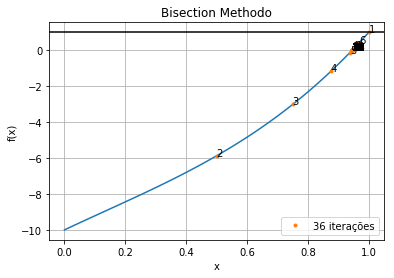
\includegraphics[scale=0.5]{/home/souza/Documents/semestre_2019-2/calculo_numerico/trabalho_1/graficos/bisection_f1.png}
    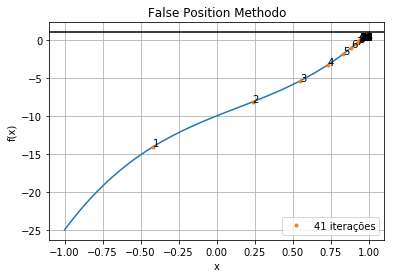
\includegraphics[scale=0.5]{/home/souza/Documents/semestre_2019-2/calculo_numerico/trabalho_1/graficos/false_position_f1.png}\\
    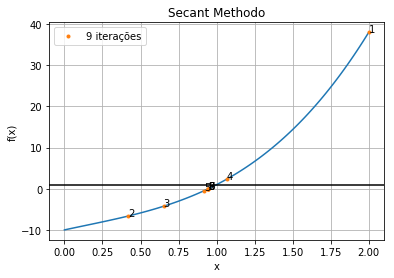
\includegraphics[scale=0.5]{/home/souza/Documents/semestre_2019-2/calculo_numerico/trabalho_1/graficos/secant_f1.png}
    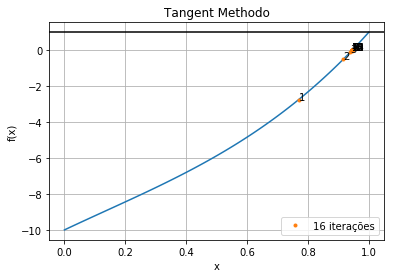
\includegraphics[scale=0.5]{/home/souza/Documents/semestre_2019-2/calculo_numerico/trabalho_1/graficos/tangent_f1.png}
    \caption{Graficos da função um executada pelos quatro metodos presentes.}
\end{figure}

\begin{figure}[!h]
    \centering
    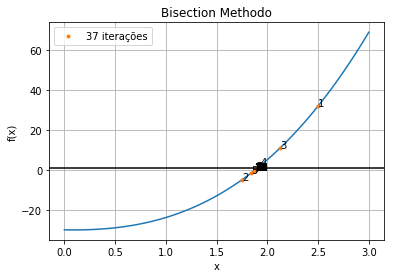
\includegraphics[scale=0.5]{/home/souza/Documents/semestre_2019-2/calculo_numerico/trabalho_1/graficos/bisection_f2.png}
    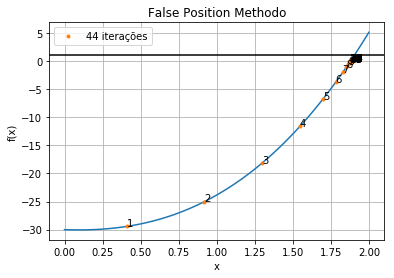
\includegraphics[scale=0.5]{/home/souza/Documents/semestre_2019-2/calculo_numerico/trabalho_1/graficos/false_position_f2.png}\\
    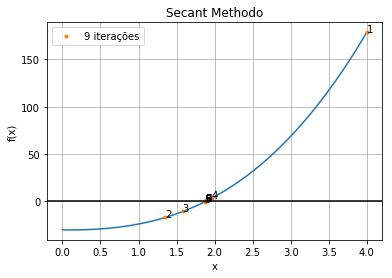
\includegraphics[scale=0.5]{/home/souza/Documents/semestre_2019-2/calculo_numerico/trabalho_1/graficos/secant_f2.png}
    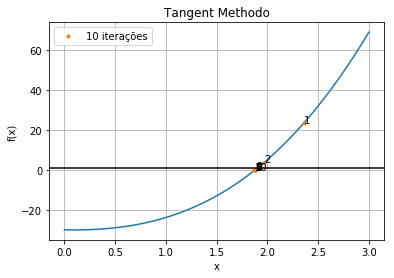
\includegraphics[scale=0.5]{/home/souza/Documents/semestre_2019-2/calculo_numerico/trabalho_1/graficos/tangent_f2.png}
    \caption{Graficos da função dois executada pelos quatro metodos presentes.}
\end{figure}

\begin{figure}[!h]
    \centering
    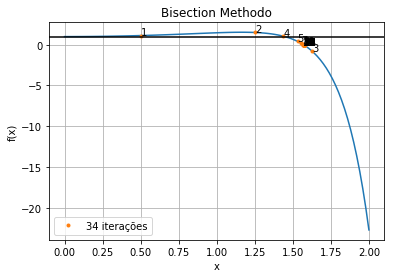
\includegraphics[scale=0.5]{/home/souza/Documents/semestre_2019-2/calculo_numerico/trabalho_1/graficos/bisection_f3.png}
    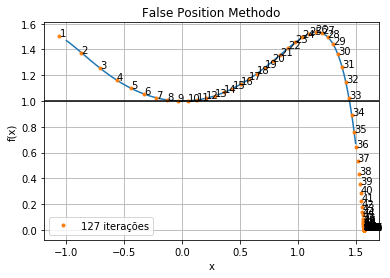
\includegraphics[scale=0.5]{/home/souza/Documents/semestre_2019-2/calculo_numerico/trabalho_1/graficos/false_position_f3.png}\\
    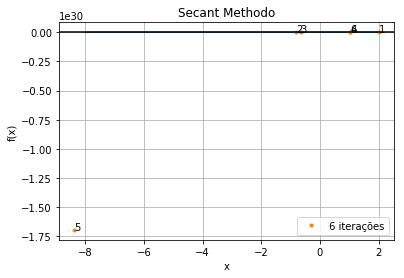
\includegraphics[scale=0.5]{/home/souza/Documents/semestre_2019-2/calculo_numerico/trabalho_1/graficos/secant_f3.png}
    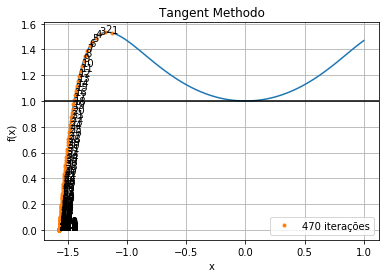
\includegraphics[scale=0.5]{/home/souza/Documents/semestre_2019-2/calculo_numerico/trabalho_1/graficos/tangent_f3.png}
    \caption{Graficos da função três executada pelos quatro metodos presentes.}
\end{figure}

\begin{figure}[!h]
    \centering
    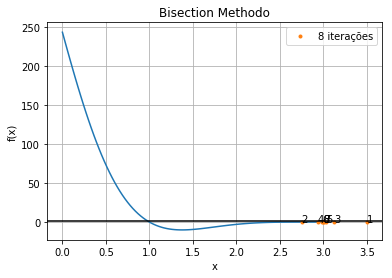
\includegraphics[scale=0.5]{/home/souza/Documents/semestre_2019-2/calculo_numerico/trabalho_1/graficos/bisection_f4.png}
    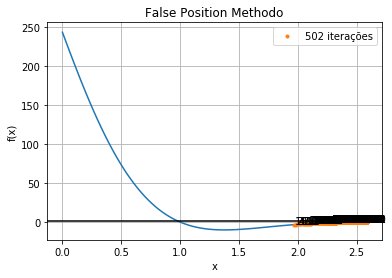
\includegraphics[scale=0.5]{/home/souza/Documents/semestre_2019-2/calculo_numerico/trabalho_1/graficos/false_position_f4.png}\\
    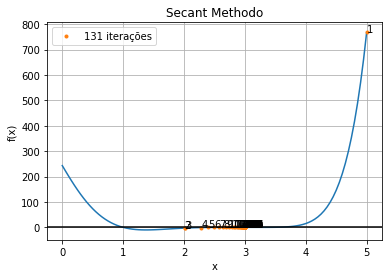
\includegraphics[scale=0.5]{/home/souza/Documents/semestre_2019-2/calculo_numerico/trabalho_1/graficos/secant_f4.png}
    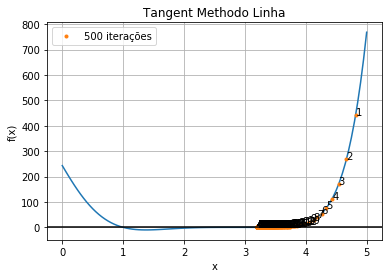
\includegraphics[scale=0.5]{/home/souza/Documents/semestre_2019-2/calculo_numerico/trabalho_1/graficos/tangent_f4.png}
    \caption{Graficos da função quatro executada pelos quatro metodos presentes.}
\end{figure}

\begin{figure}[!h]
    \centering
    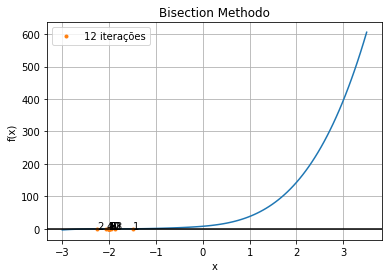
\includegraphics[scale=0.5]{/home/souza/Documents/semestre_2019-2/calculo_numerico/trabalho_1/graficos/bisection_f5.png}
    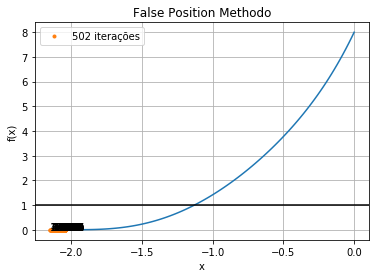
\includegraphics[scale=0.5]{/home/souza/Documents/semestre_2019-2/calculo_numerico/trabalho_1/graficos/false_position_f5.png}\\
    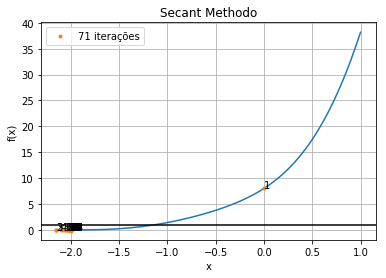
\includegraphics[scale=0.5]{/home/souza/Documents/semestre_2019-2/calculo_numerico/trabalho_1/graficos/secant_f5.png}
    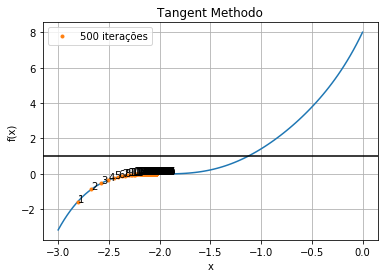
\includegraphics[scale=0.5]{/home/souza/Documents/semestre_2019-2/calculo_numerico/trabalho_1/graficos/tangent_f5.png}
    \caption{Graficos da função cinco executada pelos quatro metodos presentes.}
\end{figure}
\end{document}
